\chapter{Own Work}
\label{chap:own_work}

Alongside the evaluation pipeline, I built a browser-based application to test and demonstrate the uncertainty estimation methods interactively. It reads the same JSON outputs that the tables in this chapter are drawn from, so any result can be explored in the interface without re-running any code. The application is described at the end of this chapter in Section~\ref{sec:web_interface}, once all the results it displays have been introduced.

% ── Experimental Setup ────────────────────────────────────────────────────────
\section{Experimental Setup and Design Decisions}
\label{sec:setup}

The evaluation is built around PatchCamelyon (PCAM) as a binary histopathology classification benchmark \cite{veeling2018rotation,pcamchallenge}, using a Vision Transformer fine-tuned for two-class prediction \cite{dosovitskiy2021image}. Four uncertainty estimation methods are compared: the confidence baseline (1-MSP), MC~Dropout, a deep ensemble of three checkpoints, and post-hoc temperature scaling. The values reported in this chapter come directly from the evaluation pipeline's JSON output files and are not post-processed by hand.

\paragraph{Method selection.} The confidence baseline (MSP) serves as reference. Temperature scaling adds post-hoc recalibration at near-zero cost. MC~Dropout and deep ensembles represent the two main practical alternatives to Bayesian inference. Comparing all four under identical conditions gives a quantitative cost-benefit picture.


\paragraph{Sample sizes.} The primary evaluation uses $n = 1024$ test patches: large enough for stable aggregate metrics while keeping the $T = 30$ MC~Dropout passes tractable on the available hardware. Shift evaluations and conformal prediction use $n = 2048$ where single forward passes suffice.

\paragraph{A training-time issue worth noting.} During training, it became clear that the learning rate needed more careful tuning than initially expected. An early run with learning rate $10^{-4}$ produced a model that achieved high training accuracy but failed to generalize---the loss oscillated after the first few hundred steps rather than converging smoothly. Dropping to $1 \times 10^{-5}$ resolved this. The configuration used for all reported models is listed in Appendix~\ref{chap:appendix}.

\paragraph{Deep ensemble construction.} All three members start from \texttt{google/vit-base-patch16-224} and are fine-tuned independently on PatchCamelyon with different training set sizes and epoch counts (Member~1: 262K samples, 2 ep; Member~2: 20K samples, 5 ep; Member~3: 10K samples, 4 ep; all at lr $= 10^{-5}$). Diversity thus comes from data subset variation rather than independent random seeds. Implications are discussed in Section~\ref{sec:limitations}.

\section{Evaluation Protocol}

The primary evaluation runs on a 1024-sample PCAM test subset with synthetic shift severities $\{1,3,5\}$. All metrics are computed by the pipeline and saved to JSON; values in this chapter are read directly from those files. The four evaluation dimensions are: predictive discrimination (accuracy, ROC AUC, sensitivity, specificity), calibration (ECE 15-bin, NLL, Brier score), uncertainty usefulness (error-detection AUROC using $1-\mathrm{MSP}$), and selective prediction (AURC). A multi-axis protocol is necessary because a model can classify accurately while being poorly calibrated, or be well calibrated while still failing to flag likely errors \cite{linmans2022ood,thagaard2020datasetshift}.

\section{In-Distribution Evaluation Results}

\begin{table}[H]
    \centering
    \caption{In-distribution test results for the implemented uncertainty methods. Lower values are better for ECE, NLL, and AURC.}
    \label{tab:id_results}
    \resizebox{\linewidth}{!}{%
    \begin{tabular}{lcccccccc}
        \toprule
        Method & Accuracy & ROC AUC & Sensitivity & Specificity & ECE $\downarrow$ & NLL $\downarrow$ & Err-det AUROC $\uparrow$ & AURC $\downarrow$ \\
        \midrule
        Confidence        & 0.8555 & \textbf{0.9647} & 0.7304 & 0.9860 & 0.0863 & 0.4203 & 0.8043 & 0.0452 \\
        MC Dropout        & 0.6855 & 0.9218 & 0.3862 & \textbf{0.9980} & 0.2377 & 1.0027 & 0.7442 & 0.1506 \\
        Deep Ensemble     & \textbf{0.8672} & 0.9601 & \textbf{0.7725} & 0.9661 & 0.0577 & \textbf{0.3352} & \textbf{0.8279} & \textbf{0.0377} \\
        Temp.\ Scaling    & 0.8555 & \textbf{0.9647} & 0.7304 & 0.9860 & \textbf{0.0496} & 0.3504 & 0.8043 & 0.0452 \\
        \bottomrule
    \end{tabular}}
\end{table}


Table~\ref{tab:id_results} shows several clear patterns. The deep ensemble leads in accuracy ($0.8672$) and sensitivity ($0.7725$); three independently fine-tuned models provide diversity that reduces false negatives. MC~Dropout is the weakest at $0.6855$ due to probability-space aggregation of the $T=30$ passes (Jensen's inequality bias, discussed in Section~\ref{sec:limitations}).

Temperature scaling achieves the best calibration (ECE $0.0496$), correcting the fine-tuned model's overconfidence ($T = 1.512$). The deep ensemble follows at ECE $0.0577$; MC~Dropout is severely miscalibrated at ECE $0.2377$; this is largely an aggregation artefact rather than an intrinsic weakness of the method --- averaging $T$ softmax vectors in probability space pushes probability mass toward $0.5$ (Jensen's inequality, see \Cref{sec:limitations}), which compresses confidence scores and breaks the alignment between predicted probability and empirical accuracy that calibration requires. In error detection, the deep ensemble leads ($0.8279$ AUROC); confidence and temperature scaling are tied at $0.8043$ since temperature scaling is rank-preserving. Adding stochastic complexity does not automatically improve the in-distribution uncertainty signal --- only ensemble diversity provides a consistent gain.

The reliability diagrams (\Cref{fig:benchmark_reliability}) confirm the calibration ordering: temperature scaling and the deep ensemble stay close to the diagonal; MC~Dropout deviates substantially as stochastic averaging compresses predictions toward 0.5. The risk-coverage curves (\Cref{fig:benchmark_risk_coverage}) mirror the same ranking (AURC: deep ensemble $0.0377$, confidence/temp.\ scaling $0.0452$, MC~Dropout $0.1506$).

\begin{figure}[H]
    \centering
    \includegraphics[width=0.78\textwidth]{figures/benchmark_reliability_comparison.png}
    \caption{Reliability diagrams for all four uncertainty methods.}
    \label{fig:benchmark_reliability}
\end{figure}

\begin{figure}[H]
    \centering
    \includegraphics[width=0.78\textwidth]{figures/benchmark_risk_coverage_comparison.png}
    \caption{Risk-coverage curves for all four uncertainty methods.}
    \label{fig:benchmark_risk_coverage}
\end{figure}

The overlap between correct and incorrect prediction uncertainty distributions is large enough that no single threshold cleanly separates safe from unsafe predictions --- this is why AUROC remains below 0.83 even for the best method.

\section{Distribution Shift and OOD Evaluation}

Because pathology systems may encounter scanner variation, compression artifacts, stain differences, and other acquisition changes, a thesis on trustworthy digital pathology should not stop at in-distribution evaluation. Following the motivation of pathology-focused uncertainty studies \cite{linmans2022ood,thagaard2020datasetshift}, the implementation also evaluates synthetic shifts generated from blur, JPEG degradation, color perturbation, and additive noise.

\begin{figure}[H]
    \centering
    \includegraphics[width=0.98\textwidth]{figures/corruption_preview.png}
    \caption{Synthetic corruption types applied to one representative patch per dataset at three severity levels. Each severity column shows one PCAM patch (blue label, lymph node histology) and one NCT-CRC patch (orange label, colorectal histology) side by side. Blur and additive noise degrade high-frequency cellular detail progressively; JPEG compression introduces blocking artefacts; colour shift (desaturation + contrast boost) alters stain appearance without removing structural information. Severity~5 represents an extreme degradation that substantially exceeds typical real-world scanner variation.}
    \label{fig:corruption_preview}
\end{figure}

\begin{table}[H]
    \centering
    \caption{Grouped shift results. Near-OOD is the mean over severity 1 and 3 conditions; far-OOD is severity 5. OOD detection AUROC separates shifted from clean samples using uncertainty scores. Evaluated on $n=256$ per condition.}
    \label{tab:shift_results}
    \resizebox{\linewidth}{!}{%
    \begin{tabular}{lcccccc}
        \toprule
        Method & Near AUROC $\uparrow$ & Near Acc. $\uparrow$ & Near ECE $\downarrow$ & Far AUROC $\uparrow$ & Far Acc. $\uparrow$ & Far ECE $\downarrow$ \\
        \midrule
        Confidence    & 0.5391 & 0.8140 & 0.0935 & 0.5414 & 0.6982 & 0.2193 \\
        MC Dropout    & 0.5027 & 0.7104 & 0.1731 & 0.4548 & 0.6074 & 0.3065 \\
        Deep Ensemble & \textbf{0.5510} & \textbf{0.8354} & \textbf{0.0693} & \textbf{0.5855} & \textbf{0.7139} & \textbf{0.1682} \\
        Temp.\ Scaling& 0.5390 & 0.8140 & 0.0898 & 0.5411 & 0.6982 & 0.1888 \\
        \bottomrule
    \end{tabular}}
\end{table}


The grouped shift results in \Cref{tab:shift_results} present a cleaner story than might be expected. Within this synthetic-shift evaluation, the deep ensemble is the strongest method on every criterion under both near- and far-OOD conditions: it maintains the highest classification accuracy ($0.8354$ near, $0.7139$ far), the best calibration, and the highest OOD-detection AUROC ($0.5510$ near, $0.5855$ far). Temperature scaling and confidence cluster closely on accuracy and AUROC, which is expected since they share the same underlying predictions.

MC~Dropout shows the steepest degradation under shift. Its far-OOD detection AUROC falls to $0.4548$---below chance---meaning the model assigns \emph{lower} uncertainty to severely corrupted inputs than to clean ones. This inverted behavior is consistent with the compress-toward-$0.5$ pathology observed in-distribution: once all predictions are already maximally uncertain, adding more corruption cannot push them further, and the uncertainty score loses its discriminative value entirely.

An important caveat: the shift evaluation uses $n=256$ per condition, smaller than the $n=1024$ used for in-distribution metrics. The OOD detection AUROCs are all within a few percentage points of $0.50$, so some variability is expected at this sample size.

\begin{table}[H]
    \centering
    \small
    \caption{ECE under synthetic distribution shift. Clean ECE is the in-distribution baseline evaluated on the same $n=256$ shift subset (10-bin ECE); sev1--sev5 are increasing corruption intensities. Clean ECE values differ from Table~\ref{tab:id_results} because that table uses 15-bin ECE on $n=1024$.}
    \label{tab:ece_shift}
    \begin{tabular}{llccccc}
        \toprule
        Shift type & Method & Clean & Sev. 1 & Sev. 3 & Sev. 5 \\
        \midrule
        Blur   & Confidence        & 0.0760 & 0.0492 & 0.2811 & 0.3763 \\
        Blur   & MC Dropout        & 0.1085 & 0.0855 & 0.3563 & 0.4124 \\
        Blur   & Deep Ensemble     & 0.0489 & 0.0363 & 0.2362 & 0.3347 \\
        Blur   & Temp.\ Scaling    & 0.0480 & 0.0637 & 0.2279 & 0.3117 \\
        \midrule
        Noise  & Confidence        & 0.0760 & 0.0774 & 0.1381 & 0.3087 \\
        Noise  & MC Dropout        & 0.1085 & 0.1606 & 0.3181 & 0.4231 \\
        Noise  & Deep Ensemble     & 0.0489 & 0.0403 & 0.0554 & 0.1578 \\
        Noise  & Temp.\ Scaling    & 0.0480 & 0.0770 & 0.1102 & 0.2707 \\
        \midrule
        JPEG   & Confidence        & 0.0760 & 0.0425 & 0.0584 & 0.1514 \\
        JPEG   & MC Dropout        & 0.1085 & 0.0969 & 0.1051 & 0.2882 \\
        JPEG   & Deep Ensemble     & 0.0489 & 0.0382 & 0.0455 & 0.1250 \\
        JPEG   & Temp.\ Scaling    & 0.0480 & 0.0441 & 0.0653 & 0.1059 \\
        \midrule
        Color  & Confidence        & 0.0760 & 0.0493 & 0.0516 & 0.0408 \\
        Color  & MC Dropout        & 0.1085 & 0.1377 & 0.1244 & 0.1021 \\
        Color  & Deep Ensemble     & 0.0489 & 0.0444 & 0.0581 & 0.0555 \\
        Color  & Temp.\ Scaling    & 0.0480 & 0.0736 & 0.0561 & 0.0670 \\
        \bottomrule
    \end{tabular}
\end{table}

Blur is the most destructive perturbation for most methods. Confidence ECE rises from $0.076$ to $0.376$ at severity 5; MC~Dropout reaches $0.412$ under blur and $0.423$ under noise at the same severity. The degradation pattern is shift-dependent: under blur the sharpest increase occurs between severity 1 and 3 (e.g.\ Confidence: $+0.232$), while under noise and JPEG the larger jump tends to fall between severity 3 and 5. Color jitter has a surprisingly small effect --- confidence ECE actually drops to $0.041$ at severity 5, possibly because H\&E stain variation in the training data already acts as implicit augmentation. Deep Ensemble and Temperature Scaling are the most robust, with JPEG and noise curves remaining flat through severity 3. MC~Dropout performs worst under blur and noise. Absolute ECE values at high severities should be treated as indicative; the mapping from synthetic corruption to clinical scanner variation is not straightforward.



\subsection{Calibration under Distribution Shift}
\label{subsec:ece_shift}

We tracked Expected Calibration Error across four corruption types (blur, additive noise, JPEG degradation, and color perturbation) at severity levels 1, 3, and 5, for all four methods. The goal was to understand not only whether calibration degrades under shift, but how quickly and whether different perturbation types affect it differently.


\begin{figure}[H]
    \centering
    \includegraphics[width=0.95\textwidth]{figures/ece_under_shift.png}
    \caption{Expected Calibration Error (ECE) as a function of corruption severity for all four methods and four shift types. Deep ensemble achieves the lowest ECE across most conditions; MC~Dropout degrades most severely under blur. The colour-jitter panel is the exception: ECE for confidence and temperature scaling \emph{decreases} at severity~5, a counterintuitive result discussed in the text.}
    \label{fig:ece_under_shift}
\end{figure}

\paragraph{Summary.} MC~Dropout does not improve on the confidence baseline for in-distribution error detection, and its accuracy drop is a larger cost than the modest uncertainty gain is worth. Deep ensembles lead on accuracy, calibration, and error-detection AUROC across both in-distribution and synthetic-shift conditions.


\section{Extended Uncertainty Analysis}
\label{sec:extended_analysis}

\subsection{Conformal Prediction}
\label{subsec:conformal}

Split conformal prediction (introduced in \Cref{sec:conformal}) converts any classifier's output into prediction sets with a finite-sample coverage guarantee. We applied it to the confidence baseline, MC~Dropout, and the deep ensemble, holding out a separate calibration split from the PCAM validation set to compute the nonconformity score quantile. Empirical coverage is simply the fraction of test samples for which the true label actually falls inside the returned prediction set; the theory guarantees this fraction is at least $1 - \alpha$.


\begin{table}[H]
    \centering
    \caption{Split conformal prediction results at three miscoverage levels. Coverage should meet or exceed the target $1-\alpha$. $\bar{s}$ is the average prediction set size (range 0--2 for binary classification). Singleton rate: fraction of predictions where only one class is returned (confident prediction). Full-set rate: fraction where both classes \{0,1\} are returned (model cannot commit). Any remainder ($1 - \text{singleton} - \text{full-set}$) are empty sets, which by definition cannot contain the true label and directly cause coverage failures.}

    \label{tab:conformal}
    \resizebox{\linewidth}{!}{%
    \begin{tabular}{llccccc}
        \toprule
        Method & $\alpha$ & Target cov. & Empirical cov. & $\bar{s}$ & Singleton rate & Full-set rate \\
        \midrule
        Confidence    & 0.05 & 0.95 & 0.9678 & 1.2856 & 0.7144 & 0.2856 \\
        Confidence    & 0.10 & 0.90 & 0.9131 & 1.1108 & 0.8892 & 0.1108 \\
        Confidence    & 0.20 & 0.80 & 0.7798 & 0.8550 & 0.8550 & 0.0000 \\
        \midrule
        MC Dropout    & 0.05 & 0.95 & 0.9585 & 1.4639 & 0.5361 & 0.4639 \\
        MC Dropout    & 0.10 & 0.90 & 0.8779 & 1.2627 & 0.7373 & 0.2627 \\
        MC Dropout    & 0.20 & 0.80 & 0.7358 & 0.9468 & 0.9468 & 0.0000 \\
        \midrule
        Deep Ensemble & 0.05 & 0.95 & 0.9673 & 1.2705 & 0.7295 & 0.2705 \\
        Deep Ensemble & 0.10 & 0.90 & 0.9141 & 1.1025 & 0.8975 & 0.1025 \\
        Deep Ensemble & 0.20 & 0.80 & 0.7856 & 0.8491 & 0.8491 & 0.0000 \\
        \bottomrule
    \end{tabular}}
\end{table}

Table~\ref{tab:conformal} shows a mixed picture. At $\alpha = 0.10$ (target coverage $0.90$), the confidence baseline ($0.9131$) and deep ensemble ($0.9141$) both satisfy the guarantee with $\approx10\%$ full-label sets. MC~Dropout falls short at $0.8779$: a one percentage-point gap that in a screening setting would exclude one true label per roughly 40 predictions. At $\alpha = 0.05$ all three exceed the target, but MC~Dropout includes both classes for $46.4\%$ of predictions, making it the least efficient. All three fail the $\alpha = 0.20$ target ($0.78$, $0.74$, $0.79$). The direct cause is empty prediction sets: at this permissive threshold the calibrated quantile falls below the minimum nonconformity score, so the predictor outputs $\mathcal{C}(x) = \emptyset$ for $14.5\%$ (confidence), $5.3\%$ (MC~Dropout), and $15.1\%$ (deep ensemble) of test inputs; an empty set cannot contain the true label and immediately counts as a coverage failure.


\begin{figure}[H]
    \centering
    \includegraphics[width=0.85\textwidth]{figures/conformal_coverage_setsize.png}
    \caption{Conformal prediction coverage (left) and average prediction-set size (right) for three methods across $\alpha$ levels. MC~Dropout is the only method that falls below the nominal coverage guarantee at $\alpha=0.10$.}
    \label{fig:conformal_coverage}
\end{figure}

\subsection{Aleatoric and Epistemic Uncertainty Decomposition}
\label{subsec:aleatoric_epistemic}

Under the MC~Dropout framework, total predictive entropy can be decomposed into an epistemic component---the mutual information between predictions and model parameters---and an aleatoric component representing irreducible data-level noise. We computed this decomposition over the PCAM test set using $T = 30$ stochastic forward passes. The decomposition was not applied to the deep ensemble: with only $M = 3$ members the epistemic mutual information estimate would be too coarse to be informative, and extending it to ensembles with larger $M$ is left as future work.


Of the total mean predictive entropy ($0.3228$ nats), only $0.0123$ nats correspond to epistemic mutual information ($3.8\%$); the remaining $96.2\%$ is aleatoric. The dominant uncertainty source in PCAM is patch-level ambiguity, not lack of model knowledge. Patches near tissue boundaries may be genuinely equivocal even to an expert pathologist, and a large, consistent training corpus keeps epistemic uncertainty low. This means collecting more data is unlikely to reduce model uncertainty meaningfully in this setting.

\begin{table}[H]
    \centering
    \small
    \caption{Aleatoric and epistemic uncertainty decomposition from MC~Dropout ($T=30$) on the PCAM test set, and their respective error-detection AUROC values.}
    \label{tab:aleatoric_epistemic}
    \begin{tabular}{lcc}
        \toprule
        Component & Mean value (nats) & Error-detection AUROC \\
        \midrule
        Total predictive entropy & 0.3228 & 0.7827 \\
        Epistemic (mutual information) & 0.0123 & 0.7414 \\
        Aleatoric & 0.3105 & 0.7844 \\
        \bottomrule
    \end{tabular}
\end{table}

\Cref{tab:aleatoric_epistemic} shows that the aleatoric component achieves a slightly higher error-detection AUROC ($0.7844$) than the epistemic component ($0.7414$), despite the common assumption that epistemic uncertainty should be more diagnostic of individual prediction errors. One possible explanation is that erroneous predictions in this setting are mostly caused by genuinely hard patches --- exactly the kind of samples that drive up aleatoric uncertainty. The epistemic component, being nearly constant at its small mean value, provides a less discriminative signal by comparison.

One caveat applies: the $T = 30$ stochastic passes with fixed dropout masks are not formal Bayesian inference over the posterior; they are an approximation, and the resulting decomposition should be treated as indicative rather than exact. With more passes or a different approximation family, the epistemic estimate might shift.

\begin{figure}[H]
    \centering
    \begin{subfigure}[b]{0.82\textwidth}
        \centering
        \includegraphics[width=\textwidth]{figures/aleatoric_epistemic_histograms.png}
        \caption{Uncertainty histograms for correct vs.\ incorrect predictions.}
        \label{fig:ae_histograms}
    \end{subfigure}

    \vspace{0.5em}

    \begin{subfigure}[b]{0.72\textwidth}
        \centering
        \includegraphics[width=\textwidth]{figures/aleatoric_epistemic_scatter.png}
        \caption{Per-sample epistemic vs.\ aleatoric uncertainty.}
        \label{fig:ae_scatter}
    \end{subfigure}
    \caption{Aleatoric and epistemic uncertainty decomposition. The vast majority of total uncertainty is aleatoric (96.2\%), with epistemic uncertainty near zero for most samples.}
    \label{fig:ae_decomposition}
\end{figure}


\subsection{Cross-Domain OOD Evaluation}
\label{subsec:cross_domain_ood}

We applied the PCAM-trained ViT to the NCT-CRC-HE-100K dataset \cite{nct_crc_kather}, a colorectal cancer histology benchmark with nine tissue classes not seen during training, using only zero-shot transfer: no retraining, no domain adaptation, and no overlap between label spaces.

\begin{figure}[H]
    \centering
    \includegraphics[width=0.72\textwidth]{figures/umap_cross_domain.png}
    \caption{UMAP projection of ViT \texttt{[CLS]} token embeddings for $n=512$ PCAM test patches (blue circles) and $n=512$ NCT-CRC-HE-100K patches (red squares). The two domains show partial separation: domain-specific clusters are visible at the periphery, but the central region contains considerable overlap. This mixed structure explains both why NCT-CRC can be considered a cross-domain shift and why the PCAM decision boundary still generalises to a large fraction of NCT-CRC patches.}
    \label{fig:umap_cross_domain}
\end{figure}

\Cref{fig:umap_cross_domain} shows that the two domains are only partially separated in the ViT feature space: domain-specific clusters appear at the periphery, but substantial overlap persists in the central region. NCT-CRC therefore occupies a mix of in-distribution-adjacent and genuinely novel feature regions. This partially-shifted structure accounts for both the non-trivial zero-shot accuracy ($84$--$88\%$) and the modest uncertainty discrimination scores reported below.


\begin{table}[H]
    \centering
    \caption{Cross-domain transfer results. Accuracy is evaluated on the binary tumor/normal decision boundary of the PCAM-trained model applied to NCT-CRC. ECE measures calibration on each domain separately. Uncertainty is $1 - \mathrm{MSP}$; the discrimination AUROC uses uncertainty to separate the two domains, treating PCAM as negative and NCT-CRC as positive --- values near $0.5$ indicate the domains are indistinguishable by uncertainty alone.}
    \label{tab:cross_domain}
    \resizebox{\linewidth}{!}{%
    \begin{tabular}{lcccccccc}
        \toprule
        Method & PCAM acc. & PCAM ECE & PCAM unc. & NCT-CRC acc. & NCT-CRC ECE & NCT-CRC unc. & Discrim.\ AUROC \\
        \midrule
        Confidence     & 0.881 & 0.0276 & 0.1059 & 0.844 & 0.0703 & 0.1066 & 0.5711 \\
        MC Dropout     & 0.768 & 0.1014 & 0.1321 & 0.793 & 0.0566 & 0.1807 & 0.6204 \\
        Deep Ensemble  & 0.861 & 0.0680 & 0.0786 & 0.875 & 0.0707 & 0.0766 & 0.5628 \\
        Temp.\ Scaling & 0.881 & 0.0367 & 0.1391 & 0.844 & 0.0465 & 0.1465 & 0.5711 \\
        \bottomrule
    \end{tabular}}
\end{table}

All four methods classify $84$--$88\%$ of NCT-CRC patches correctly zero-shot (MC~Dropout is the exception at $79\%$, its accuracy penalty carrying over from in-distribution inference), which suggests that the binary decision boundary learned on PCAM transfers reasonably well to colorectal tissue. Calibration on NCT-CRC is broadly comparable to PCAM: ECE values are within a few percentage points for confidence, deep ensemble, and temperature scaling; MC~Dropout actually shows lower ECE on NCT-CRC ($0.057$) than on PCAM ($0.101$), likely because its systematic compression-toward-$0.5$ happens to align better with the less confident predictions the cross-domain data demands.

The uncertainty discrimination results (Discrim.\ AUROC) indicate that none of the methods reliably distinguishes the two domains by uncertainty score alone. Values range from $0.563$ to $0.620$, all close to chance. MC~Dropout is the only method where mean uncertainty is higher on NCT-CRC ($0.181$) than on PCAM ($0.132$); the deep ensemble shows the opposite --- lower uncertainty on NCT-CRC ($0.077$ vs.\ $0.079$). These patterns are consistent with the known tendency of ensembles to become overconfident when members agree in low-ambiguity regions outside the training distribution \cite{linmans2022ood} --- a failure mode visible here precisely because the UMAP confirms that part of the NCT-CRC manifold falls in sparsely-populated feature regions where the ensemble members happen to agree.

\Cref{fig:cross_domain_rel_rc} provides a deeper view through reliability diagrams and risk-coverage (RC) curves for the confidence baseline and MC~Dropout. Both reliability diagrams show that the model is overconfident on NCT-CRC in the low- and high-confidence bins: the NCT-CRC curve (dashed) lies below the PCAM curve across most confidence ranges and drops clearly below the perfect-calibration diagonal at the extremes (confidence $\approx 0.55$: accuracy only $0.44$; confidence $\approx 0.94$: accuracy $0.90$), meaning the model assigns high confidence to predictions that are correct less often than expected. This confirms the calibration gap reflected in the ECE values and explains why lower mean uncertainty is possible alongside lower accuracy. The RC curves reinforce this: deferring the most uncertain predictions (leftmost part of the curve) reduces error on PCAM much more steeply than on NCT-CRC, indicating that uncertainty scores are a weaker proxy for error on the cross-domain data.

\begin{figure}[H]
    \centering
    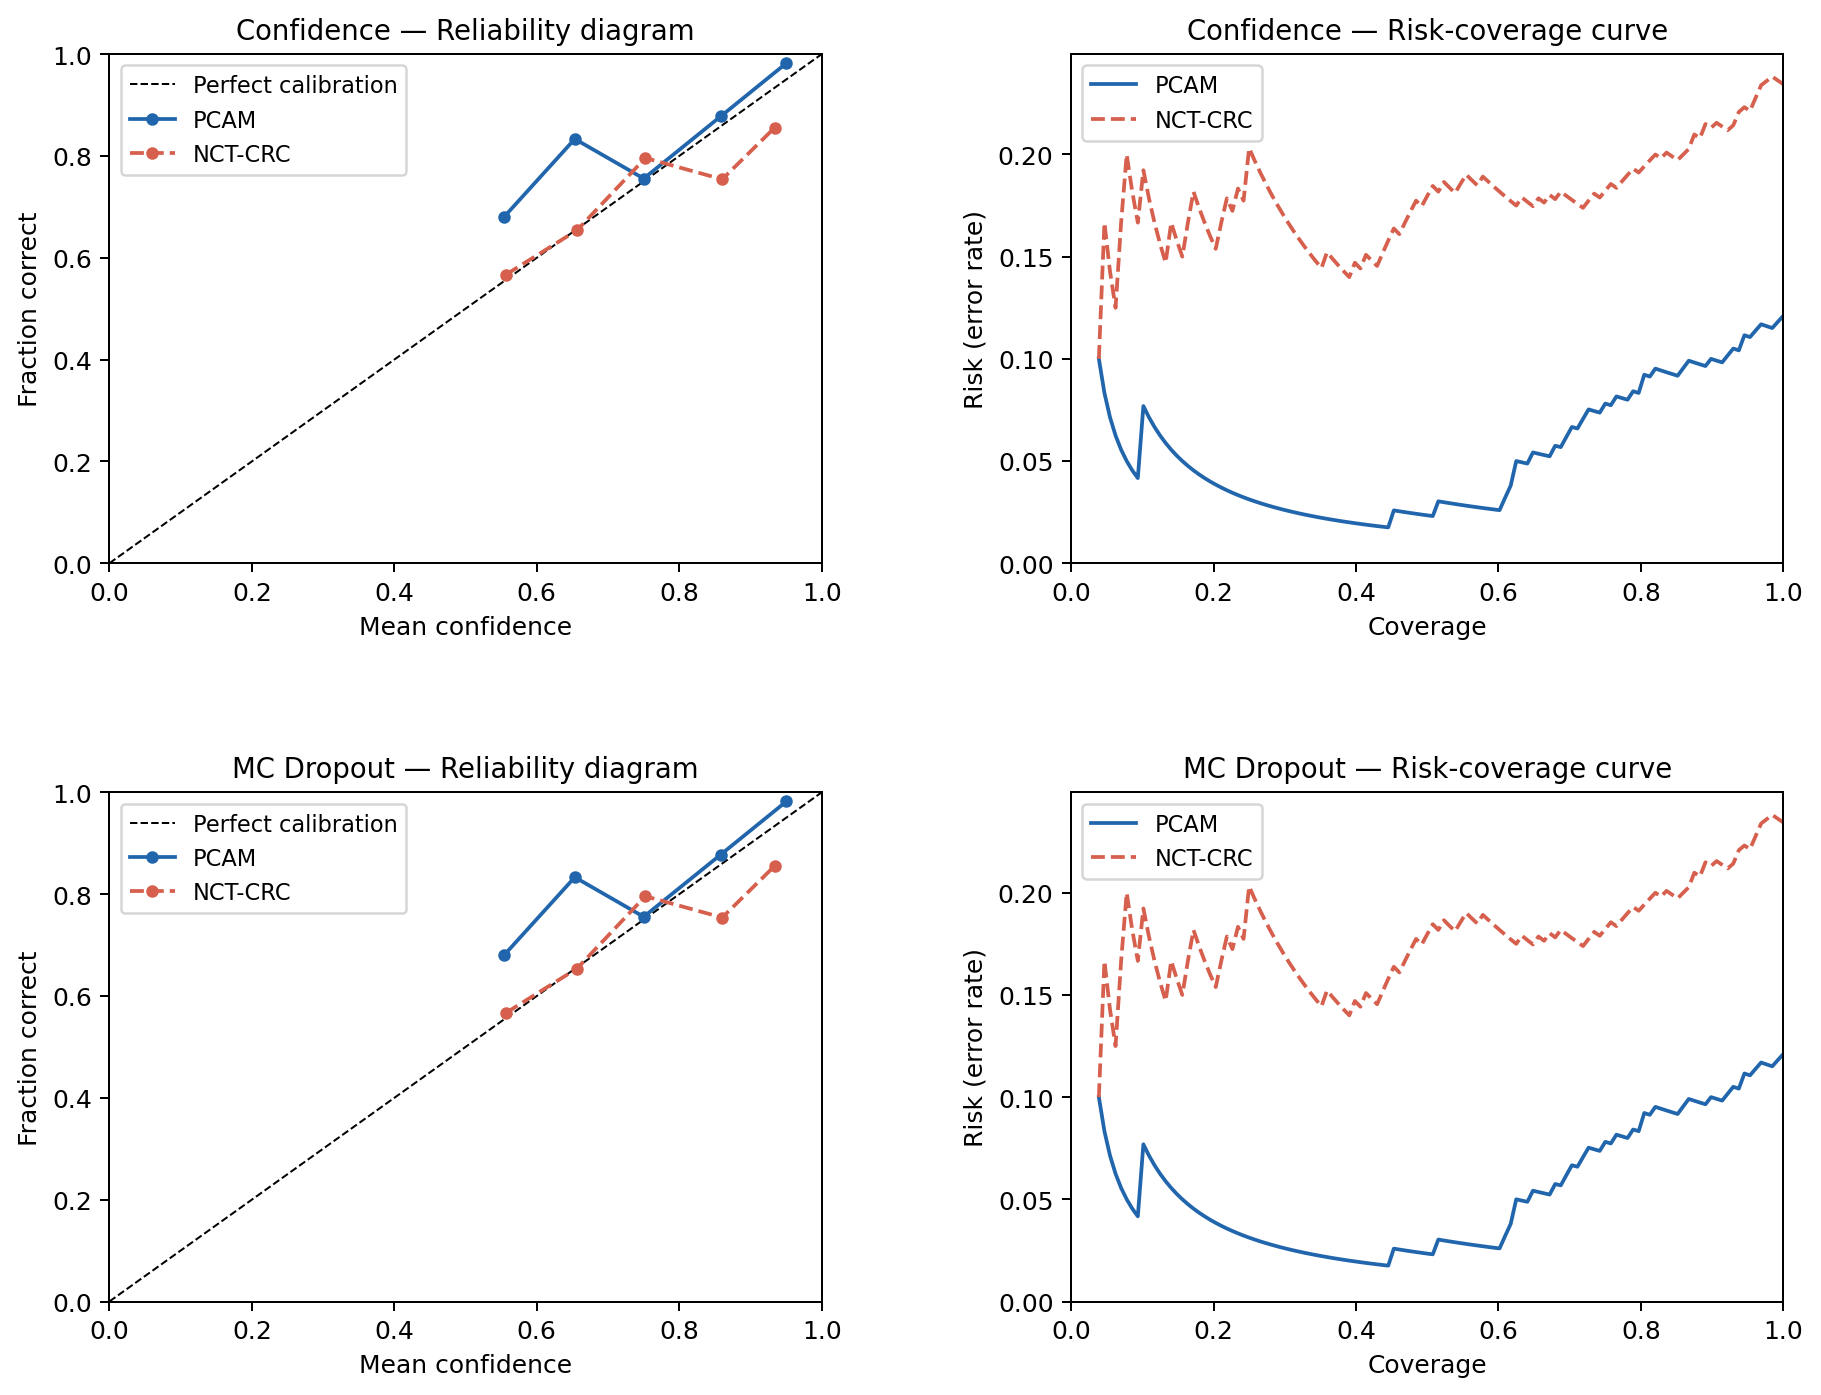
\includegraphics[width=\textwidth]{figures/cross_domain_reliability_rc.png}
    \caption{Reliability diagrams (left column) and risk-coverage curves (right column) for the confidence baseline (top row) and MC~Dropout (bottom row), comparing PCAM test patches (solid blue) with NCT-CRC-HE-100K patches (dashed red), each evaluated on $n=256$ samples. Reliability diagrams plot mean confidence per bin against the fraction of correct predictions; the dashed diagonal marks perfect calibration. RC curves plot error rate as a function of coverage when predictions are ordered by confidence (most confident retained first); a well-calibrated uncertainty estimate should produce a steeply declining RC curve.}
    \label{fig:cross_domain_rel_rc}
\end{figure}




% ── Limitations and Future Work ──────────────────────────────────────────────
\section{Limitations and Future Work}
\label{sec:limitations}


Several aspects of the current work constrain how strongly the conclusions can be generalized. The most important are the sample size, the probability-space aggregation used for MC~Dropout, and the limited diversity of the ensemble; each is discussed in turn, followed by directions for future work. A recurring theme is that strong performance on in-distribution and synthetic-shift criteria provides no guarantee on cross-domain OOD detection: the deep ensemble leads on every synthetic-shift criterion yet assigns \emph{lower} uncertainty on NCT-CRC than on PCAM, which is precisely why a multi-criteria evaluation protocol is necessary.

\paragraph{Sample size.} Primary metrics are computed on $n = 1024$ test patches. Under the normal approximation to the binomial, this gives a 95\% confidence interval of $\pm 1.96\sqrt{\hat{p}(1-\hat{p})/n} \approx \pm 3$~pp on accuracy (worst case at $\hat{p}=0.5$). Differences of 1--2~pp between methods therefore fall within the margin of error and should not be over-interpreted; the 17~pp MC~Dropout gap is large enough to be robust, but the 1--2~pp gaps between confidence, temperature scaling, and the deep ensemble are not.

\paragraph{MC~Dropout aggregation.} The 17.0~pp accuracy drop ($0.8555 \rightarrow 0.6855$) stems from probability-space aggregation: averaging softmax outputs $\frac{1}{T}\sum_t \operatorname{softmax}(f_t(x))$ rather than logit-space averaging $\operatorname{softmax}\!\left(\frac{1}{T}\sum_t f_t(x)\right)$. By Jensen's inequality, the former produces a distribution that is flatter (closer to uniform) than the softmax of the mean logits, which is why confidence collapses under $T=30$ stochastic passes. Probability-space averaging is not simply wrong: it is the natural formulation of the Bayesian model average and preserves the probabilistic interpretation of the mixture. Logit-space averaging avoids the Jensen bias and typically recovers accuracy, but the result is no longer a formal mixture of predictive distributions. The deep ensemble uses the same probability-space formula (Eq.~\ref{eq:ensemble_mean}), yet does not suffer an analogous accuracy drop, because the $M=3$ members produce genuinely divergent logits --- so their softmax average is still peaked --- whereas MC~Dropout passes through the same network with random masks produce correlated, low-magnitude logit differences that compound into a strong bias toward $0.5$ when averaged. Results throughout this thesis are reported with the probability-space implementation.

\paragraph{Ensemble diversity and temperature scaling.} Ensemble members share the same ImageNet-21k pre-trained backbone and differ only in training subset size, not random seed. This choice was deliberate: with a large frozen feature extractor, different random seeds for the linear head alone would produce nearly identical representations, so data-subset variation was used to introduce meaningful diversity in what each member has seen. The resulting diversity is nonetheless weaker than the standard Lakshminarayanan protocol~\cite{lakshminarayanan2017simple}, which trains from independently randomised initialisations, and this contributes to the OOD overconfidence on NCT-CRC. Temperature scaling ($T = 1.512$) corrects in-distribution overconfidence effectively but does not protect against calibration degradation under severe image corruption.

\paragraph{Future directions.} Three natural extensions follow from the above limitations. First, switching to logit-space MC~Dropout aggregation with $T \geq 100$ would provide a fairer comparison by removing the Jensen bias entirely. Second, energy-based or dedicated OOD detection heads~\cite{liu2020energy} could push beyond the $0.62$ OOD-detection AUROC ceiling observed in the cross-domain evaluation. Third, mondrian conformal prediction~\cite{vovk2005algorithmic} would provide per-class coverage guarantees rather than the marginal guarantee evaluated here, which is more informative in class-imbalanced clinical settings.


% ── Web Interface ─────────────────────────────────────────────────────────────
\section{Web Interface}
\label{sec:web_interface}

To make the evaluation results accessible and reproducible beyond static tables, I built a browser-based application that serves as an interactive front end to the uncertainty estimation pipeline. The tool lets a user load any evaluation bundle, browse dataset patches, launch training runs, and explore all result panels --- calibration, conformal prediction, aleatoric/epistemic decomposition, and cross-domain OOD detection --- without touching the command line or re-running any experiment.

\subsection{Architecture}

The application runs as a local Flask server with plain HTML and JavaScript on the front end --- no build toolchain required. Figure~\ref{fig:web_arch} shows its overall structure. The backend serves three categories of data: dataset images read directly from H5 files, pre-computed evaluation results from \texttt{evaluation/*.json}, and live training output streamed back to the browser via Server-Sent Events.


\begin{figure}[H]
\centering
\begin{tikzpicture}[
    font=\small,
    box/.style={rectangle, draw, rounded corners=3pt, minimum width=3.0cm, minimum height=0.75cm, align=center, fill=gray!10},
    store/.style={rectangle, draw, rounded corners=3pt, minimum width=2.8cm, minimum height=0.65cm, align=center, fill=blue!8},
    arr/.style={-{Stealth}, thick},
    darr/.style={<->, thick, dashed},
]

% Browser
\node[box, fill=green!10] (browser) at (-1,0) {Browser\\(HTML / JS)};

% Flask
\node[box, fill=orange!12] (flask) at (4.5,0) {Flask App\\\texttt{web/app.py}};

% Three data stores
\node[store] (evaljson) at (8.5, 1.4) {Evaluation JSONs\\\texttt{evaluation/*.json}};
\node[store] (h5)       at (8.5, 0)   {Dataset H5 files\\\texttt{data/raw/}};
\node[store] (ckpt)     at (8.5,-1.4) {Checkpoints\\\texttt{checkpoints/}};

% uncertainty_lab below flask
\node[box, fill=purple!8] (ulab) at (4.5,-2.2) {\texttt{uncertainty\_lab}\\(metrics, pipeline)};

% Arrows browser <-> flask
\draw[darr] (browser) -- node[above, font=\footnotesize]{REST / SSE} (flask);

% Flask -> stores
\draw[arr] (flask) -- (evaljson);
\draw[arr] (flask) -- (h5);
\draw[arr] (flask) -- (ckpt);

% Flask <-> ulab
\draw[darr] (flask) -- node[right, font=\footnotesize]{train / eval} (ulab);
\draw[arr]  (ulab)  -- (ckpt);

\end{tikzpicture}
\caption{High-level architecture of the web application. The browser communicates with Flask over REST and Server-Sent Events. Flask reads pre-computed evaluation JSONs and dataset image files directly; training jobs are delegated to the \texttt{uncertainty\_lab} pipeline and their output is streamed back live.}
\label{fig:web_arch}
\end{figure}

\subsection{Dataset Page}

The Dataset page (Figure~\ref{fig:ui_dataset}) shows a label integrity check alongside a configurable sample browser for both PCAM and NCT-CRC-HE-100K patches. A separate panel shows what any selected patch looks like after each of the four synthetic image degradations used to simulate distribution shift --- Gaussian blur, additive noise, JPEG-like downsampling, and colour jitter --- at all three severity levels; this was the main way I verified the corruption parameters before running the evaluations.


\begin{figure}[H]
    \centering
    \includegraphics[width=0.95\textwidth]{figures/ui_sample_browser.png}
    \caption{The Dataset page sample browser showing PCAM training patches. Each tile is labelled with its ground-truth class. The toolbar supports dataset switching (PCAM / NCT-CRC-HE-100K), split selection, label filtering, and offset or random sampling modes.}
    \label{fig:ui_dataset}
\end{figure}

\subsection{Run Page}

The Run page (Figure~\ref{fig:ui_run}) is a training console that exposes key hyperparameters, streams training output live via Server-Sent Events, and records completed runs in a persistent table with validation accuracy and configuration.

\begin{figure}[H]
    \centering
    \begin{subfigure}[b]{0.95\textwidth}
        \centering
        \includegraphics[width=\textwidth]{figures/ui_run_train.png}
        \caption{Training configuration form with live log output area.}
        \label{fig:ui_run}
    \end{subfigure}
    \vspace{0.5em}
    \begin{subfigure}[b]{0.95\textwidth}
        \centering
        \includegraphics[width=\textwidth]{figures/ui_run_history.png}
        \caption{Previous runs table showing model checkpoints with their validation accuracy and training configuration.}
        \label{fig:ui_run_history}
    \end{subfigure}
    \caption{The Run page. The training form (top) accepts hyperparameters and streams live log output. Completed runs (bottom) are listed with their validation accuracy; any checkpoint can be selected as the evaluation target on the Results page.}
\end{figure}

\subsection{Results Page}

The Results page loads a pre-computed evaluation bundle from a dropdown; the canonical bundle covers all four uncertainty estimation methods on the PCAM test split. Results are split into sections for standard metrics, reliability diagrams, risk--coverage curves, conformal prediction (Figure~\ref{fig:ui_conformal}), aleatoric/epistemic decomposition and ECE-under-shift (Figure~\ref{fig:ui_eval_results}), and cross-domain OOD detection (Figure~\ref{fig:ui_ood_shift}).


\begin{figure}[H]
    \centering
    \includegraphics[width=0.95\textwidth]{figures/ui_conformal.png}
    \caption{Conformal prediction panel on the Results page. The left plot shows empirical vs.\ target coverage for all three methods across $\alpha \in \{0.05, 0.10, 0.20\}$; the right plot shows prediction set sizes (efficiency). MC Dropout falls below the target coverage line at $\alpha = 0.10$ and $\alpha = 0.20$.}
    \label{fig:ui_conformal}
\end{figure}

\begin{figure}[H]
    \centering
    \includegraphics[width=0.88\textwidth]{figures/ui_eval_results.png}
    \caption{Advanced uncertainty analysis panels. Top: aleatoric vs.\ epistemic decomposition showing that 96.2\% of total uncertainty is aleatoric, with a per-sample scatter plot colored by prediction correctness. Bottom: ECE-under-shift table for all four methods across blur, noise, JPEG, and color corruptions at severities 1, 3, and 5, with color-coded degradation.}
    \label{fig:ui_eval_results}
\end{figure}

\begin{figure}[H]
    \centering
    \includegraphics[width=0.95\textwidth]{figures/ui_ood_shift.png}
    \caption{Cross-domain OOD detection panel. Each row reports the mean uncertainty on PCAM (in-distribution) and NCT-CRC (out-of-distribution) samples, together with the OOD AUROC for distinguishing the two domains using uncertainty as a signal. Deep Ensemble shows inverted behavior (lower uncertainty on OOD data), while MC Dropout achieves the best OOD AUROC of 0.620.}
    \label{fig:ui_ood_shift}
\end{figure}
